\documentclass[times,10pt,twocolumn]{article}
\usepackage[portuguese]{babel}
\usepackage{reportASE}
\usepackage{times}
\usepackage{enumitem}
\usepackage[utf8]{inputenc}
\usepackage{graphicx}
\usepackage{hyperref}
\usepackage{xcolor}
\usepackage{listings}
\definecolor{goodBlue}{RGB}{70, 123, 182}
\lstset{
	basicstyle=\ttfamily\footnotesize,
	showstringspaces=false,
	commentstyle=\color{red},
	keywordstyle=\color{black}
}
\usepackage[portuguese,ruled,noend]{algorithm2e} 
\pagestyle{empty}


%------------------------------------------------------------------------- 
\begin{document}

\title{
	Sensor Network for Animal Husbandry
	\\
	\large Software for Embedded Systems -- Instituto Superior Técnico
	\\
	\normalsize{Grupo 9 - Tagus}
}

\author{
	Alexandre Filipe Campos\\ alexandre.t.campos@ist.utl.pt\\n.º 66354	}

\maketitle
\thispagestyle{empty}


%-------------------------------------------------------------------------
\begin{abstract}
Os desafios enfrentados pela agricultura moderna nunca foram tão grandes. Sempre houve a necessidade de os produtores de gado terem capacidade de observar os animais o mais frequentemente possível. Mas gerir uma grande quantidade de animais, enquanto ao mesmo tempo permiti-los ser tão soltos quanto possível, não é uma tarefa fácil. Recentemente, temos visto o aumento do uso de redes de sensores sem fio para ajudar no manejo dos animais. 

Ao colocar um nó sensor num animal que pode controlar a sua localização, a sua interação com os outros, ou a sua saúde, entre outros parâmetros. E podemos ter uma contínua, durante todo o dia, observação dos animais e, portanto, podemos intervir o mais cedo possível, se alguma situação ocorra. 

O objetivo deste projeto é criar esses nós sensores em uma rede.
 
\end{abstract}


%------------------------------------------------------------------------- 
\section*{Introdução}
%------------------------------------------------------------------------- 
\section{Descrição geral do sistema}

O sistema é descrito pelas seguintes principais funcionalidades:

\begin{itemize}
	\item Monitorização da localização GPS dos animais
	\item Monitorização do consumo de comida do animais
	\item Capacidade de difusão de mensagens
	\item Configuração dos níveis de consumo de comida
	\item Configuração dos níveis de comida disponível 
\end{itemize}

Cada nó possui uma placa de sensor que permite a anexação de um módulo GPS. Este módulo irá providenciar leituras para a constante monitorização da posição dos animais. Adicionalmente todos os nós terão um RFID (Radio-Frequency IDentification') token para permitir definir a a proximidade aos vários pontos de alimentação presentes. Em cada nó é guardada a informação sobre o consumo máximo diário de comida para cada animal e a quantidade de comida que já consumiu no dia.

Os locais de alimentação irão suportar a alimentação dos animais ao despenderem uma dose controlado de comida para o animal, caso este ainda não tenha ultrapassado o seu limite diário. Os locais de alimentação serão munidos de um leitor RFID para detetar a presença do animal e identificar o animal aquando da aproximação deste. Adicionalmente terão um módulo Rádio-Frequência para a comunicação de quanta comida a dispensar ao animal.

Todas as medidas colecionadas pelos nós serão difundidas periodicamente através do módulo RF (Rádio Frequência). Para demonstrar toda a funcionalidade do sistema e do protocolo de encaminhamento foi definida uma topologia para a representação geográfica dos animais que permite que a qualquer momento esteja sempre um nó perto do servidor que controla a rede e efectua a coleção dos dados. Os nós mais distantes do servidor terão as suas mensagens encaminhadas pelos outros nós da rede, havendo sempre mais do que uma caminho possível para efeitos de redundância.

No servidor será possível monitorizar e configurar os diversos parâmetros através de comandos. Como efetuar alterações de consumos diários de comida a nós individuais ou todos os nós.

%-------------------------------------------------------------------------
\section{Arquitetura do Sistema}


%-------------------------------------------------------------------------
\subsection{Arquitectura de Hardware}

A rede \textit{wireless} de sensores é constituída por um conjunto de nós – \textit{MICAz motes}. Estes módulos são especialmente concebidos para criar redes de sensores \textit{wireless} de baixo consumo energético (figura \ref{fig:micaz}).

\begin{figure}[h]
	\centering
	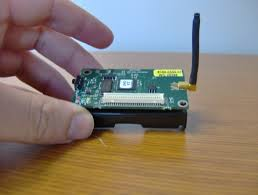
\includegraphics[width=0.3\textwidth]{micaz.jpeg}	
	\caption{MICAz mote}
	\label{fig:micaz}
\end{figure}

O transmissor rádio, opera na largura de banda dos 2.4GHz e tem uma taxa de transmissão de dados de 250 kbps. Para mais informações, é possível consultar respectiva \textit{datasheet}\cite{micaz}.


Para poder colecionar dados de localização GPS, é necessário ligar ao \textit{MICAz}, uma placa de sensor e uma antena GPS compatível. Para esse efeito foi escolhida a MTS420 sensor board (Figura \ref{fig:mts420}) que tem disponível diversos sensores entre eles GPS.  

\begin{figure}[h]
	\centering
	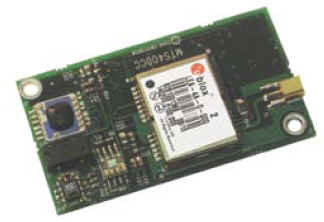
\includegraphics[width=0.30\textwidth]{Mts420.jpg}	
	\caption{MTS420 - \textit{Sensor board}}
	\label{fig:mts420}
\end{figure}

Uma possível implementação considerada para suportar os pontos de alimentação seria o use de um Arduíno (Figura \ref{fig:ard}). Este iria ser munido de um módulo RF 2.4Ghz para ser possível comunicar com os micaz motes e de um RFID Reader para detetar a proximidade do animal. 

\begin{figure}[h]
	\centering
	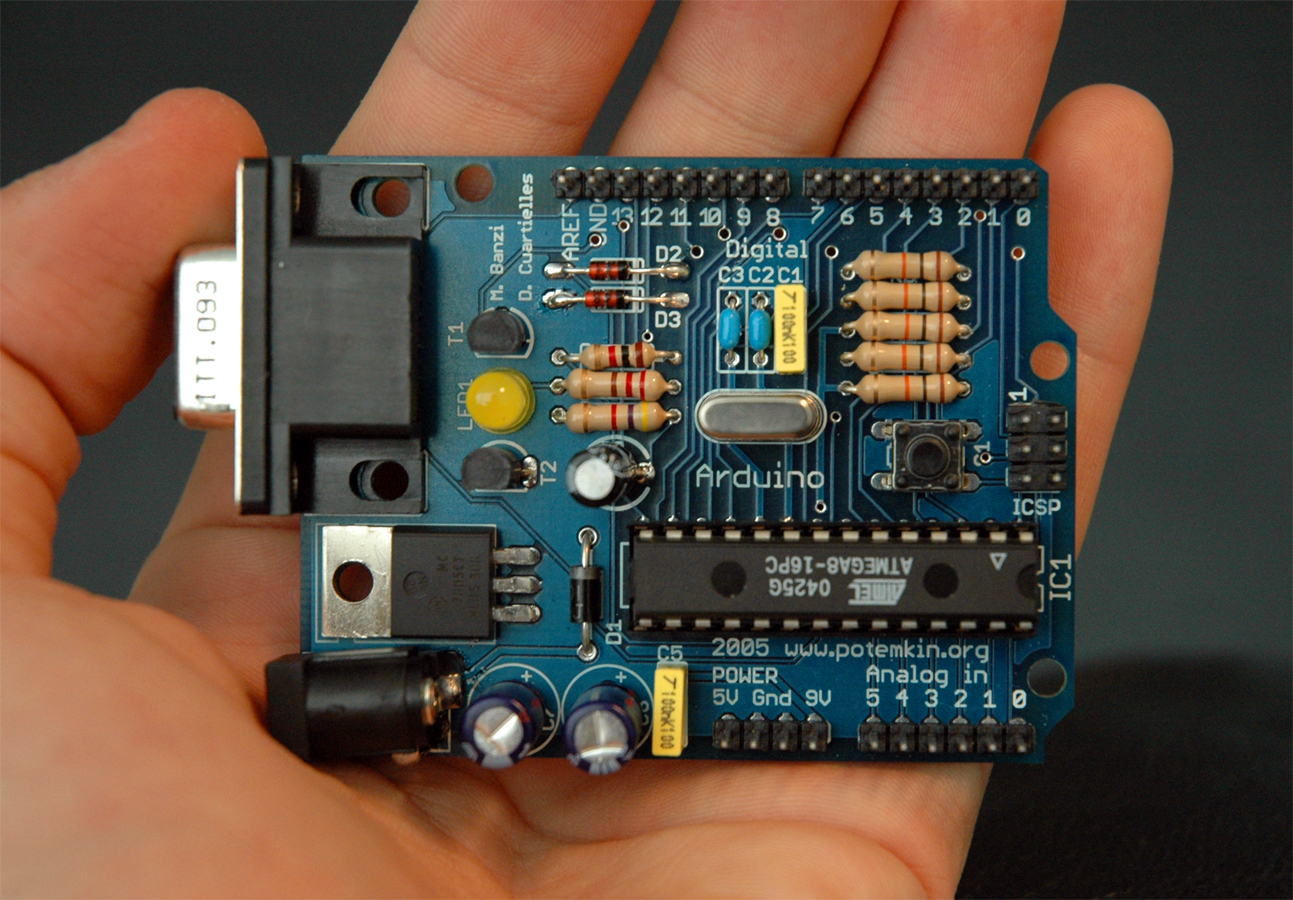
\includegraphics[width=0.30\textwidth]{ard.jpg}	
	\caption{\textit{Arduíno}}
	\label{fig:ard}
\end{figure}

Para auxiliar no dispenso da comida com alguma precisão de quantidade podemos ligar ao arduíno um Servo Motor (Figure \ref{fig:servo}) que com base na quantidade de comida configurada no mote do animal poderá rodar e abrir uma espécia de fúnil para a queda de comida, um certo ângulo durante um certo tempo para servir a quantidade certa.

\begin{figure}[h]
	\centering
	
\includegraphics[width=0.30\textwidth]{servo.jpg}	
	\caption{Servo motor}
	\label{fig:servo}
\end{figure}
	
%-------------------------------------------------------------------------
\subsection{Arquitectura de Software}

O sistema foi desenhado e desenvolvido para o sistema operativo \textit{TinyOS}, integralmente implementado na linguagem \textit{nesC}. O \textit{TinyOS} é um sistema operativo baseado em eventos, composto por uma arquitetura de componentes. Fazendo uso do simulador TOSSIM para simular a totalidade da aplicação. 
		
%-------------------------------------------------------------------------	
\subsubsection{Componentes}
	
A aplicação é suportada pelos seguintes componentes principais:

\begin{itemize}
	\item Módulo: \textit{AnimalC} 
	\item Configuração: \textit{AnimalAppC}
\end{itemize}	

Toda a lógica está presente no módulo \textit{AnimalC}, que gere todo o funcionamento do sensor desde comunicação com outros nós e \textit{feeding spots} a interação com o sensor GPS. Este módulo faz uso de interfaces disponibilizadas pelo \emph{tinyOS} como \emph{ActiveMessageC} (responsável pelo controlo da comunicação rádio), \emph{TimerMilliC} (que permite temporizar diversas acções), \emph{DemoSensorC} (que oferece a interface de ligação a vários sensores). As ligações entres estes e o módulo são feitas pela configuração \emph{AnimalAppC}.

Mais específicamente o módulo TimerMilliC é utilizado para temporizar diversos aspectos da aplicação, sendo estes, a verificação de proximidade a um feeding spot. Esta proximidade é simulada através de uma variável booleana que está constantemente a ser verificada. Assim que é detectada a sua activação (esta acção simula a deteção do badge RFID pelo local de alimentação e posterior comunicação rádio com o mote), é despoletada a alimentação do animal. Outro aspecto da aplicação que é controlado é a temporização é a leitura do GPS e comunicação dos dados do nó (GPS e comida). O componente DemoSensorC representa um dispositivo sensor genérico que permite simular vários sensores, sendo usado nesta caso para simular a leitura GPS.


%-------------------------------------------------------------------------
\subsubsection{Lógica de Execução}

Assim que um nó é iniciado a interface \emph{Boot } é sinalizada sendo despoletado o event \emph{booted()}, aqui é dada a inicialização a várias variáveis e também iniciado a componente rádio.

Assim que a componente rádio é iniciada com sucesso, são iniciados os três componentes periódicos (disponibilizados pelo componente \emph{TimerMilliC}, que oferecem ao nó a autonomia para ler os sensores periodicamente, comunicar informação dos sensores e verificar proximidade a um ponto de alimentação.

Assim que o evento temporizado para a leitura de GPS dispara são chamadas os métodos da interface esperada mas a sua implementação é simulada com a leitura de um ficheiro. Assim que a leitura está completa, é guardada e não será enviada até que o evento de envio de informação dispare. 

A mesma lógica é aplicada à alimentação do animal. Através do servidor é possível injectar um pacote na rede para definir um animal como próximo de um ponto de alimentação. Esta alteração irá despoletar uma série de eventos assim que o temporizador para alimentação disparar e verificar que a proximidade é verdade. Assim que isto acontece é simulada a comunicação rádio com o ponto de alimentação através da leitura e escrita de um ficheiro.

Através da interface rádio são definidas funções especificadas para a receção das mensagens (\emph{ReceiveUpdateFoodDailyDosage.receive(..)} \& emph{ReceiveUpdateFeedingSpot.receive(...)}) de atualização da comida diária máxima e atualização da comida máxima disponível nos pontos de alimentação. A primeira será reencaminhada por todos os nós e com dois tipos de destino (todos ou um nó em especifico) e irá servir para atualizar os valores. A segunda será reencaminhada por todos os nós até que seja encontrado um que esteja próximo de um ponto de alimentação cuja mensagem seja destinada. Mais uma vez essa interação (nó próximo <--> ponto de alimentação) será simulada através do acesso a um ficheiro.

A lógica de receção e reencaminhamento de mensagens será explicada em mais detalhe na próxima secção.
	

%------------------------------------------------------------------------- 	
%\subsection{Interacção entre Software e Hardware}


%------------------------------------------------------------------------- 
\section{Arquitectura da Rede}
\label{sec:rede}

Os nós que compõem a rede \textit{wireless} de sensores encontram-se distribuídos segundo uma topologia estabelecida através de um ficheiro que indica quais os nós que recebem uma dada mensagem transmitida por outro nó e o respectivo ganho, em dB. A figura \ref{fig:topo} ilustra a topologia utilizada no contexto deste projecto.

A topologia da rede de sensores é estabelecida através de um ficheiro (topo.txt) presente no projecto. Este ficheiro representa as ligações entre nós e o respectivo ganho (em dB):

\begin{lstlisting}[language=bash]
0  1 -53.0
1  0 -54.0
1  2 -54.0
2  1 -55.0
2  3 -55.0
3  2 -55.0
3  4 -55.0
4  3 -55.0
4  5 -54.0
5  4 -53.0
5  6 -56.0
6  5 -55.0
6  7 -53.0
7  6 -52.0
7  8 -54.0
8  7 -54.0
8  9 -54.0
9  8 -55.0
9  0 -54.0
0  9 -53.0
\end{lstlisting}

O resultado é a seguinte topologia:

\begin{figure}[h]
	\hspace{-0.5cm}
	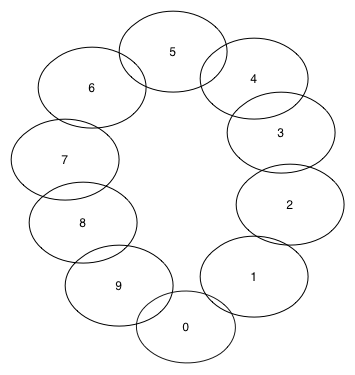
\includegraphics[width=0.46\textwidth]{topo.png}	
 	\caption{Topologia da rede de sensores}
	\label{fig:topo}
\end{figure}

O protocolo definido para a comunicação entre os nós foi uma variação \emph{broadcast flood}, em que cada nó retransmite todas as mensagens que recebe exceto alguns casos específicos: caso a mensagem seja direcionada a ele próprio, por exemplo, uma alteração da quantidade de comida máxima diária que o animal pode comer leva a que todos os cuja a mensagem não seja destinada irão fazer retransmissão em broadcast até que a mensagem chegue ao destino. Visto que todas as mensagens têm um identificador único cada nó apenas retransmite a mensagem uma vez, levando assim à conclusão que caso existam \emph{N} nós na rede a mensagem irá ser retransmitida \emph{N} vezes.

Embora este protocolo seja algo ineficiente em termos energéticos é extremamente eficaz em situações de perdas de mensagens causadas por colisões e/ou interferências de ruído, devido à elevada redundância. Outro ponto a favor é o facto de os animais possam estar em constante movimento levando assim a que a implementação de um algoritmo de encaminhamento mais sofisticado pode levar a resultados piores numa rede em constante alteração.

\subsection{Tipos de Mensagens}

Para a disseminação de informação GPS e comida dos nós foi criada a seguinte mensagem (AnimalInfo) que é disseminada periodicamente entre todos os nós com o intuito de chegar ao servidor. Cumprindo assim o objectivo ser possível aceder à informação mais recente possível sobre nós que se possam afastar da rede principal sendo impossível comunicar com eles. Desta forma também é evitado que pedidos feitos pelo servidor possam gerar uma tempestade de mensagens em resposta ao pedido.

\begin{lstlisting}[language=c++]
typedef nx_struct AnimalInfo {
  nx_int32_t gps_la; //gps latitue
  nx_int32_t gps_lo; //gps longitude
  nx_uint16_t food_g; //food eaten
  nx_uint32_t msg_id; //unique
  nx_uint16_t mote_id; //the unique mote_id
} AnimalInfo;
\end{lstlisting}

As duas seguintes mensagens não são criadas por nós mas sim injectadas na rede pelo servidor ao nó mais próximo para disseminar. Podem ter intuito de chegar a um nó específico ou no caso de destino ser zero para chegar a todos os nós ou feeding spots.

\begin{lstlisting}[language=c++]
typedef nx_struct UpdateFeedingSpot {
  nx_uint16_t food_g; //food in grams
  nx_uint32_t msg_id; //unique
  nx_uint8_t spot_id; //spot id
} UpdateFeedingSpot;
\end{lstlisting}

\begin{lstlisting}[language=c++]
typedef nx_struct UpdateFoodDailyDosage{
  nx_uint32_t msg_id; //to denie rebroadcast
  nx_uint16_t mote_dest; //if 0 deliver to all
  nx_uint8_t new_food_max; //new max amount of daily food 
} UpdateFoodDailyDosage;
\end{lstlisting}


%------------------------------------------------------------------------- 
\section{Manual de Utilização do Simulador}

Para manipular o simulador é necessário um \textit{script} em \textit{Python}, que recorre ao TOSSIM\footnote{TinyOS SIMulator} para simular a presença de vários nós sensores e outras funcionalidades. Para executar a aplicação com sucesso basta seguir os seguintes passos:

\begin{enumerate}
	\item Iniciar um terminal e colocar-se na diretoria do projecto
	\item Compilar o programa através da Makefile. Sendo o primeiro argumento o tipo de mote e o terceiro a indicar que é uma simulação.
	\begin{lstlisting}[language=bash]
make micaz sim
	\end{lstlisting}
	Este comando deverá gerar diversos ficheiros.
	\item A simulação faz uso de diversos ficheiros auxiliares que necessitam de estar presentes:
	\begin{itemize}
		\item Topologia da rede: \textit{topo.txt}
		\item Modelo de ruído: \textit{noise.txt}
		\item Simulação GPS: \textit{gps1 gps2 ... gpsN}
		\item Simulação Feeding Spot \textit{fs1 fs2 ... fsN}
	\end{itemize}
\end{enumerate}

Assim que o projecto estiver compilado com sucesso e os ficheiros todos presentes, pode-se correr o projecto com o seguinte comando:

\begin{lstlisting}[language=bash]
python server.py
\end{lstlisting}

Assim que o simulação é iniciada será questionado sobre a quantidade de nós que quer na rede. De seguida os nós serão iniciados. Assim que a iniciação terminar será presenciado com um terminal interativo que pode receber os seguintes comandos:

\begin{lstlisting}
- h                                                            *** for help
- get <mote_id> (FOR DEBUG)              *** get state info of mote
- exit                              			       *** to exit
- read <mote_id>                                     *** get last known GPS and food info
- updateFood <mote_id> <amount>        *** to update daily food. mote_id 0 for all
- getSpotFood <spot_id>                         *** to get amount of food left in feeding spot.
- updateSpotFood <spot_id> <amount>  *** to update the spots food. 0 for all.
- prox <mote_id>                                     *** turn on proximity simulation to feeding spot.
\end{lstlisting}

%------------------------------------------------------------------------- 
\section{Problemas/Soluções na Implementação}

Um dos principais problemas ao conceber a solução foi lidar com a perda de mensagens e tentar construir algo superior ao modelo de controlo de concorrência nas comunicações radio sugerido pelo tutoriais do \emph{tinyOS}. Este modelo sugere o uso de uma variável booleana a proteger a ocupação do rádio para transmissão levando a que possíveis envios (reacções a mensagens recebidas) fossem descartados. Foi então tentado desenvolver uma solução com locks distribuídos (usando mutex) que se revelou um falhanço devido a constantes situações de erro devido a \emph{deadlock} distribuído. Devido ao consumo de tempo da não resolução destes problemas a solução foi abandonada e foi decido fazer uso do modelo originalmente sugerido.

Foi contemplada também a possibilidade de implementação de algorítmo de encaminhamento mais sofisticado, mas devido à natureza da rede e comportamentos imprevisíveis (possível movimento constante dos nós) poderia revelar-se mais custoso e ineficiente em várias situações.

%------------------------------------------------------------------------- 
\section{Conclusões}

%No geral considera-se que o projecto foi bem sucedido, na medida em que todos os requisitos foram implementados usando soluções satisfatórias e tomou-se ainda a liberdade de acrescentar funcionalidades que  se consideram úteis no contexto real. Nomeadamente, a possibilidade de possuir uma rede de sensores com configurações heterogéneas, permitindo que cada sensor atenda às necessidade específicas de cada planta num cenário com diversos tipos de plantas diferentes.

%Os maiores desafios foram a adaptação ao ambiente de desenvolvimento do \textit{TinyOS} e à sua arquitectura de componentes e a selecção e integração teórica do \textit{software} com os componentes de \textit{hardware}.


%------------------------------------------------------------------------- 
\begin{thebibliography}{99}  

\bibitem{nesc}
David Gay, Philip Levis, David Culler, Eric Brewer, \textit{nesC 1.3 Language Reference Manual}, July 2009
\\http://nesl.ee.ucla.edu/fw/torres/home/projects/tossim
\_gumstix/root/nesc-1.3.1/doc/ref.pdf

\bibitem{mda}
MDA300 Data Acquisition Board Datasheet, Memsic
\\http://www.memsic.com/userfiles/files/Datasheets/
WSN/6020-0052-04\_a\_mda300-t.pdf

\bibitem{micaz}
MICAz Datasheet, ZigBee\texttrademark Alliance, Crossbow,
\\http://www.openautomation.net/uploadsproductos/
micaz\_datasheet.pdf

\bibitem{tos}
TinyOS Tutorials - TinyOS Documentation Wiki
\\http://docs.tinyos.net/tinywiki/index.php/
TinyOS\_Tutorials


\end{thebibliography}

\end{document}

%deadlocks distribuidos
%algoritmo de encaminhamento mais sofisticado abandonado devido a possibilidade e imprisivibilidade de comportamento da rede poderia levar a ser mais custoso e pouco eficiente